% !TEX program = xelatex
% 编译方式：xelatex 数学建模与实验课程设计.tex （连续编译两次以生成目录）
\documentclass[zihao=5,a4paper]{ctexart}

\usepackage{amsmath,amssymb}
\usepackage{graphicx}
\usepackage{geometry}
\usepackage{booktabs}
\usepackage{array}
\usepackage{multirow}
\usepackage{caption}
\usepackage{float}
\usepackage{listings}
\usepackage{xcolor}
\usepackage{enumitem}
\usepackage{bm}

\geometry{a4paper,left=2.5cm,right=2.5cm,top=2.5cm,bottom=2.5cm}

% ===== 按写作规范：一级标题小四黑体，正文五号宋体（zihao=5 已设正文五号） =====
\ctexset{
  section   = {format=\zihao{-4}\heiti, aftername=\quad},
  subsection= {format=\zihao{5}\heiti, aftername=\quad}
}

\captionsetup{font=small,labelsep=quad}

% ===== 代码样式 =====
\definecolor{codegreen}{rgb}{0,0.5,0}
\definecolor{codegray}{rgb}{0.5,0.5,0.5}
\definecolor{codepurple}{rgb}{0.58,0,0.82}
\definecolor{backcolour}{rgb}{0.97,0.97,0.97}

\lstset{
  basicstyle=\ttfamily\footnotesize,
  backgroundcolor=\color{backcolour},
  commentstyle=\color{codegreen},
  keywordstyle=\color{blue},
  stringstyle=\color{codepurple},
  numberstyle=\tiny\color{codegray},
  numbers=left,
  numbersep=6pt,
  breaklines=true,
  breakatwhitespace=false,
  showstringspaces=false,
  frame=single,
  rulecolor=\color{gray!60},
  tabsize=2,
  columns=fullflexible,
  keepspaces=true,
  upquote=true,
  xleftmargin=1.2em
}

\newcommand{\dd}{\,\mathrm{d}}

\begin{document}

% ============================================================
% 封面
% ============================================================
\begin{titlepage}
\centering
\vspace*{2cm}
{\zihao{-0}\heiti 合肥工业大学}\\[0.4cm]
{\zihao{0}\heiti 课\quad 程\quad 设\quad 计}\\[3.5cm]
{\zihao{3}\songti
\renewcommand{\arraystretch}{2.0}
\begin{tabular}{r@{\ }l}
设计题目 & \underline{\makebox[8cm]{\zihao{-2}\songti 数学建模与实验课程设计}}\\
学生姓名 & \underline{\makebox[8cm]{张致远}}\\
学\qquad 号 & \underline{\makebox[8cm]{2023213980}}\\
专业班级 & \underline{\makebox[8cm]{信息与计算科学23-1班}}\\
指导教师 & \underline{\makebox[8cm]{苏敏}}\\
\end{tabular}}\\[2.5cm]
{\zihao{3}\songti 2026 年 \qquad 6月 \qquad 1日}
\vfill
\end{titlepage}

% ============================================================
% 任务书
% ============================================================
\thispagestyle{empty}
\noindent{\zihao{3}\heiti 合肥工业大学课程设计任务书}
\vspace{0.8em}

\setlength{\tabcolsep}{5pt}
\renewcommand{\arraystretch}{1.4}
\noindent\begin{tabular}{|>{\centering\arraybackslash}m{1.1cm}|>{\centering\arraybackslash}m{8.8cm}|>{\centering\arraybackslash}m{1.1cm}|>{\centering\arraybackslash}m{2.8cm}|}
\hline
\shortstack{设计\\题目}\rule[-0.6cm]{0pt}{1.5cm} & 数学建模与实验课程设计 & 成\,绩 & \\\hline
\multicolumn{1}{|>{\centering\arraybackslash}m{1.1cm}|}{\shortstack{课\\程\\设\\计\\主\\要\\内\\容}} &
\multicolumn{3}{p{13.4cm}|}{%
\begin{minipage}[t][9.3cm][t]{12.9cm}
\setlength{\parindent}{0pt}
\small\noindent 本课程设计围绕《数学建模与实验》课程的七个核心专题展开，要求针对每个专题
的典型案例完成"问题分析—模型假设—模型建立—模型求解—结果分析"的完整建模流程，
并使用 MATLAB / C++ / Python 等工具上机实现与验证。具体内容包括：\par
（1）差分方程建模：贷款偿还、人口 Logistic 增长、导弹追踪等；\par
（2）微分方程建模：导弹追踪解析解、修正 Malthus 模型、捕食—食饵（Lotka--Volterra）模型；\par
（3）插值与拟合：Lagrange 插值、三次样条、曲线/曲面拟合、最小二乘；\par
（4）蒙特卡罗模拟：随机投点求面积与积分、排队系统仿真；\par
（5）线性/非线性/多目标规划：生产计划、选址、飞行管理、Pareto 前沿；\par
（6）图论建模：最短路（设备更新）、minimax 选址、最大流；\par
（7）概率统计建模：吸收马氏链、多元回归、判别分析。
\end{minipage}} \\\hline
\multicolumn{1}{|>{\centering\arraybackslash}m{1.1cm}|}{\shortstack{指\\导\\教\\师\\评\\语}} &
\multicolumn{3}{p{13.4cm}|}{%
\begin{minipage}[t][5cm][t]{12.9cm}
\setlength{\parindent}{0pt}
\small\noindent 建议：从学生的工作态度、工作量、设计（论文）的创造性、学术性、实用性及书面表达能力等方面给出评价。
\vfill
\hfill 签名：\makebox[3cm]{}\quad 2026 年 \quad 月 \quad 日\quad\quad
\end{minipage}} \\\hline
\end{tabular}

\newpage

% ============================================================
% 目录
% ============================================================
\thispagestyle{empty}
\tableofcontents
\newpage

% ============================================================
% 正文
% ============================================================

% ------------------------------------------------------------
\section{数模1差分方程建模}
% ------------------------------------------------------------

\subsection{题目 1：贷款问题}
某消费者购房需贷款 $30$ 万元，期限 $30$ 年，贷款年利率 $5.1\%$，采用固定额度还款方式，
求每月应还款额。

\textbf{问题分析与模型假设：} 每月末还款，贷款利率不变。每月总欠款满足
"上月欠款 $\times(1+$月利率$)$ 减去当月还款"。月利率 $r$ 由
$(1+r)^{12}=1+5.1\%$ 确定，得 $r=0.4233361659\%$。

\textbf{模型建立：} 记 $y_n$ 为第 $n$ 个月的总欠款，$x$ 为月还款额，$N=360$ 为期数，
$Q=300000$ 为贷款总额，则
\[
\begin{cases}
y_n=(1+r)y_{n-1}-x, & n=1,2,\dots,N,\\
y_0=Q.
\end{cases}
\]
递推展开得
\[
y_n=(1+r)^n y_0-x\,\frac{(1+r)^n-1}{r}.
\]
由全部还清条件 $y_N=y_{360}=0$ 解得
\[
x=\frac{(1+r)^N Q\,r}{(1+r)^N-1}=1625.17\ \text{元},\qquad
s=xN=585061.2\ \text{元}.
\]

\begin{lstlisting}[language=Matlab]
clc, clear, format long g
Q = 300000; r = 0.0042333616592649115; N = 360;
x = round((1+r)^N*Q*r/((1+r)^N-1), 2)   % 每月还款额
s = x*N                                  % 总还款额
format                                   % 恢复短小数显示格式
\end{lstlisting}

\subsection{题目 2：再论美国人口增长模型}
以 $\Delta t$ 年为步长，记 $x_k$ 为 $t=k$ 时人口数量（百万）。若人口增长服从
Logistic 规律，则
\[
x_{k+1}-x_k=r\,(1-s x_k)\,x_k\,\Delta t,
\]
其中 $r$ 为固有增长率，$s$ 为阻滞系数。整理为非线性一阶差分方程
\[
x_{k+1}=(1+\Delta t\,r-\Delta t\,s r\,x_k)x_k=\alpha x_k+\beta x_k^2,
\quad \alpha=1+\Delta t\,r,\ \beta=-\Delta t\,s r<0.
\]
取 $\Delta t=10$，以线性最小二乘拟合得 $\alpha=1.209489,\ \beta=-0.000413$，
$2010$ 年人口预测值为 $307.6464$ 百万。

\begin{lstlisting}[language=Matlab]
x_data = [3.9,5.3,7.2,9.6,12.9,17.1,23.2,31.4,38.6,50.2,62.9,76.0,...
          92.0,106.5,123.2,131.7,150.7,179.3,204.0,226.5,251.4];
% 构造最小二乘方程组
y   = x_data(2:end)';      % 响应向量 x_{k+1}
x_k = x_data(1:end-1)';    % 自变量 x_k
A = [x_k, x_k.^2];         % 设计矩阵
theta = A \ y;             % 参数估计 [alpha; beta]
alpha = theta(1); beta = theta(2);
fprintf('拟合结果: alpha = %.6f, beta = %.6f\n', alpha, beta);
x_pred = A * theta;        % 拟合值
figure; plot(y, 'bo'); hold on; plot(x_pred, 'r--');
xlabel('时间步 k'); ylabel('x_{k+1}'); legend('实际值','拟合值');
title('最小二乘拟合效果'); grid on;
\end{lstlisting}

\begin{figure}[H]
\centering
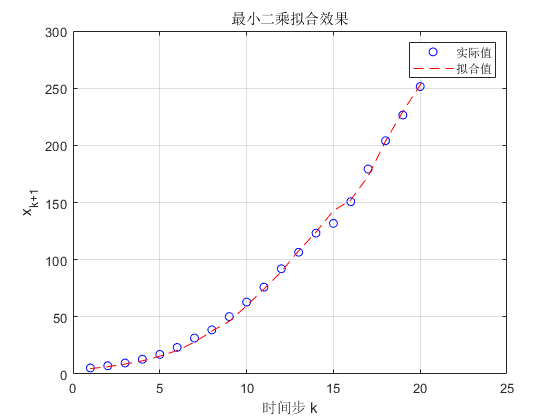
\includegraphics[width=0.62\textwidth]{figs/p1-003-000.png}
\caption{美国人口 Logistic 模型最小二乘拟合效果}
\end{figure}

\subsection{题目 3：目标跟踪问题（差分模型）}
位于原点的甲舰向 $Q_0(1,0)$ 处乙舰发射导弹，导弹始终对准乙舰。乙舰以速度 $v_0$
沿平行于 $y$ 轴方向行驶，导弹速度为 $5v_0$，求导弹运行曲线及乙舰被击中时行驶的距离。

\textbf{模型建立：} 将导弹 $P$、乙舰 $Q$ 视为质点。任意时刻导弹方向指向乙舰，则
$P(t+\Delta t)-P(t)=5v_0\,\widehat{PQ}(t)\,\Delta t$，
$Q(t+\Delta t)-Q(t)=(0,v_0\Delta t)$。取 $\Delta t=5\times10^{-5},\,v_0=1$ 模拟，
得乙舰被击中时行驶距离约 $0.2083$，总时间约 $0.2083$。

\begin{lstlisting}[language=Matlab]
v0 = 1; dt = 5e-5; threshold = 1e-4;
P = [0, 0]; Q = [1, 0]; t = 0; trajectory = P;
while true
    d = norm(Q - P);
    if d < threshold, break; end
    direction = (Q - P) / d;        % 导弹移动方向（单位向量）
    P = P + 5 * v0 * dt * direction;% 更新导弹位置
    Q(2) = Q(2) + v0 * dt;          % 乙舰沿 y 轴移动
    trajectory = [trajectory; P];
    t = t + dt;
end
fprintf('乙舰被击中时的行驶距离：%.4f\n', Q(2));
fprintf('总时间：%.4f\n', t);
figure; plot(trajectory(:,1), trajectory(:,2), 'b-'); hold on;
plot(Q(1), Q(2), 'ro','MarkerSize',10,'MarkerFaceColor','r');
xlabel('x'); ylabel('y'); title('导弹跟踪轨迹');
legend('导弹轨迹','击中位置'); grid on; axis equal;
\end{lstlisting}

\begin{figure}[H]
\centering
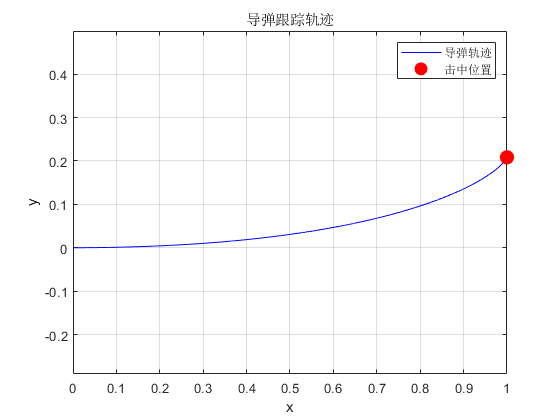
\includegraphics[width=0.55\textwidth]{figs/p1-006-001.png}
\caption{导弹跟踪轨迹（$v_0=1$，击中点约 $(1,0.21)$）}
\end{figure}

\subsection{题目 4：导弹跟踪问题（拓展）}
导弹基地正北 $120$ km 处有敌艇以 $90$ km/h 向正东行驶，基地发射导弹（$450$ km/h）
自动导航跟踪。以基地为原点、$x$ 轴指向正东、$y$ 轴指向正北，敌舰位置
$Q(t)=(vt,120)$。

\textbf{模型建立：} 记导弹在 $t_k$ 时位置 $P(x_k,y_k)$，
$\overrightarrow{PQ}=(vt_k-x_k,\,120-y_k)$，$d_k=\sqrt{(vt_k-x_k)^2+(120-y_k)^2}$，则
\[
\begin{cases}
x_{k+1}=x_k+u\cdot\dfrac{vt_k-x_k}{d_k}\Delta t,\\[2mm]
y_{k+1}=y_k+u\cdot\dfrac{120-y_k}{d_k}\Delta t,\\[2mm]
t_{k+1}=t_k+\Delta t,
\end{cases}
\qquad x_0=y_0=t_0=0.
\]
取 $\Delta t=10^{-5}$ h，命中阈值 $\varepsilon=10^{-3}$ km，迭代得命中时间
$t\approx0.2778$ h（约 $16.67$ 分钟），命中位置 $(25.0000,120.0000)$ km。
与解析解 $T=\dfrac{Du}{u^2-v^2}=\dfrac{120\times450}{450^2-90^2}\approx0.2778$ h 一致。

\begin{lstlisting}[language=Matlab]
clc, clear, format long g
v = 90; u = 450; D = 120; h = 1e-5; eps = 1e-3;
x = 0; y = 0; t = 0; trajectory = [x, y];
while true
    qx = v * t; qy = D;
    pq = [qx - x, qy - y]; d = norm(pq);
    if d < eps, break; end          % 命中
    x = x + u * pq(1)/d * h;
    y = y + u * pq(2)/d * h;
    t = t + h;
    trajectory = [trajectory; x, y];
end
fprintf('命中时间 t = %.6f h (约 %.2f 分钟)\n', t, t*60);
fprintf('命中位置 (x, y) = (%.4f, %.4f) km\n', x, y);
fprintf('敌舰沿 x 行驶距离 = %.4f km\n', v*t);
\end{lstlisting}

\begin{figure}[H]
\centering
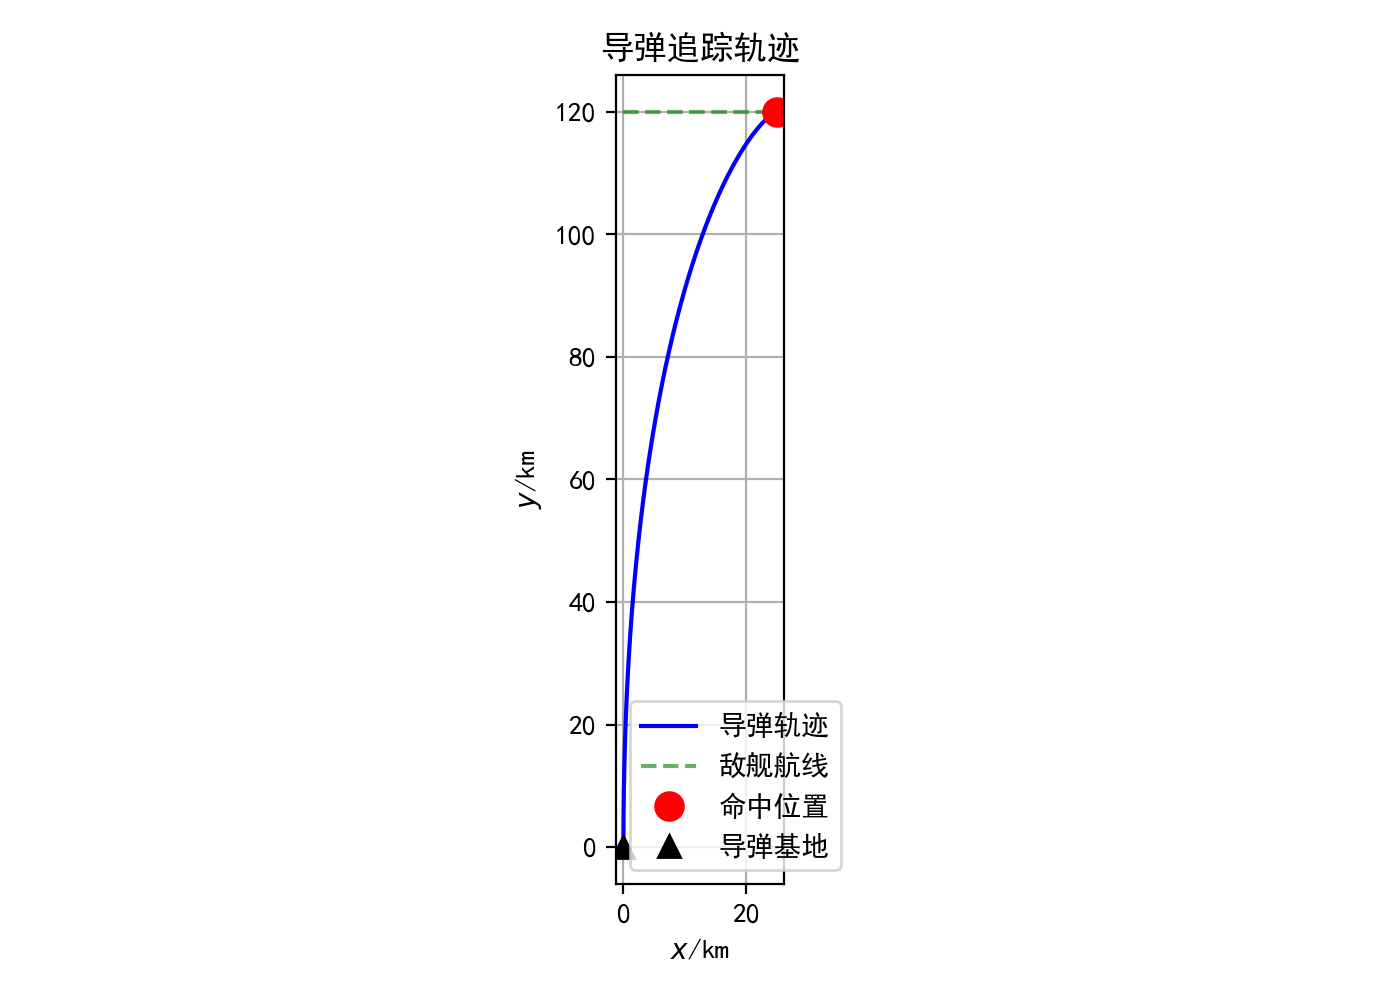
\includegraphics[width=0.4\textwidth]{figs/p1-009-002.png}
\caption{导弹追踪轨迹（命中点 $(25,120)$ km）}
\end{figure}

% ------------------------------------------------------------
\section{数模2微分方程建模}
% ------------------------------------------------------------

\subsection{题目 1：目标跟踪问题（微分模型）}
设定同第 1 节题目 3。导弹路程为乙舰路程的 $5$ 倍，故弧长满足
\[
\int_0^x\sqrt{1+(y')^2}\dd x=5v_0t.
\]
导弹轨迹切线过乙舰 $(1,v_0t)$，得 $v_0t=y+(1-x)y'$。两式分别对 $x$ 求导并令 $p=y'$：
\[
\sqrt{1+p^2}=5(1-x)\frac{\dd p}{\dd x}
\;\Longrightarrow\;
\frac{\dd p}{\sqrt{1+p^2}}=\frac{\dd x}{5(1-x)}.
\]
积分并代入 $x=0,p=0$（$C=0$）得 $p+\sqrt{1+p^2}=(1-x)^{-1/5}$，化简
\[
p=\frac12\Big[(1-x)^{-1/5}-(1-x)^{1/5}\Big].
\]
再积分并代入 $x=0,y=0$ 定常数：
\[
y=\frac12\Big[-\tfrac54(1-x)^{4/5}+\tfrac56(1-x)^{6/5}\Big]+\frac{5}{24}.
\]
令 $x=1$ 得 $y=\dfrac{5}{24}$，即乙舰行驶 $\dfrac{5}{24}$ 时被击中，$t=\dfrac{5}{24v_0}$。

\subsection{题目 2：鲑鱼}
鲑鱼服从 Malthus 增长 $\dfrac{\dd p}{\dd t}=0.003p$；鲨鱼捕食速率 $0.001p^2$，
另有每分钟 $0.002$ 条离开。

\textbf{（1）修正模型：}
\[
\frac{\dd p}{\dd t}=0.003p-0.001p^2-0.002,\qquad p(0)=10^6.
\]
\textbf{（2）平衡分析：} 令右端为零，$0.001p^2-0.003p+0.002=0$，即 $p^2-3p+2=0$，
得平衡点 $p_0=1$ 或 $p_0=2$。由于初值 $p(0)=10^6$ 远大于平衡点，负反馈项 $-0.001p^2$
使数量迅速下降；$t\to\infty$ 时趋于低水平稳定状态，可能灭绝或接近灭绝。

\subsection{题目 3：捕食—食饵模型}
\[
\frac{\dd x}{\dd t}=rx-axy,\qquad
\frac{\dd y}{\dd t}=-dy+bxy,
\]
$x(0)=20,\,y(0)=4$，$r=1,a=0.1,d=0.5,b=0.02$。用四阶 Runge--Kutta（\texttt{ode45}）
求解，给出种群随时间变化与相轨线（极限环），并计算一个周期内的平均密度
（理论上 $\bar x=d/b=25,\ \bar y=r/a=10$）。

\begin{lstlisting}[language=Matlab]
r = 1; a = 0.1; d = 0.5; b = 0.02; x0 = 20; y0 = 4;
tspan = [0, 50];
[t, sol] = ode45(@(t,y) prey_predator(t,y,r,a,d,b), tspan, [x0; y0]);
x = sol(:,1); y = sol(:,2);
figure; plot(t,x,'b','LineWidth',1.5); hold on; plot(t,y,'r','LineWidth',1.5);
xlabel('时间 t'); ylabel('种群密度');
legend('食饵 x(t)','捕食者 y(t)'); title('食饵-捕食者种群变化'); grid on;
figure; plot(x,y,'g','LineWidth',1.5);
xlabel('食饵种群 x'); ylabel('捕食者种群 y'); title('相轨线图（极限环）'); grid on;
T_index = find(x > x0, 1); T = t(T_index);
x_avg = trapz(t(1:T_index), x(1:T_index)) / T;
y_avg = trapz(t(1:T_index), y(1:T_index)) / T;
disp(['平均食饵密度: ', num2str(x_avg)]);
disp(['平均捕食者密度: ', num2str(y_avg)]);

function dydt = prey_predator(~, y, r, a, d, b)
    dydt = [r*y(1) - a*y(1)*y(2); -d*y(2) + b*y(1)*y(2)];
end
\end{lstlisting}

\begin{figure}[H]
\centering
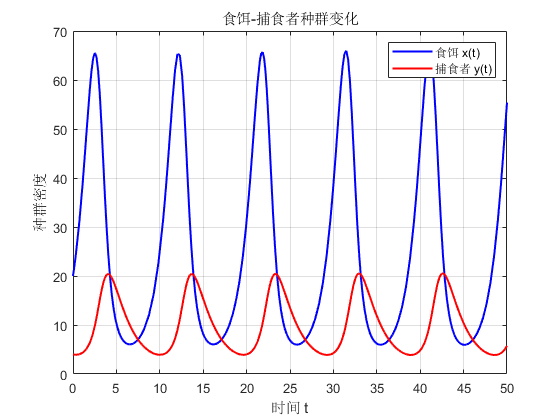
\includegraphics[width=0.49\textwidth]{figs/p2-004-000.png}
\hfill
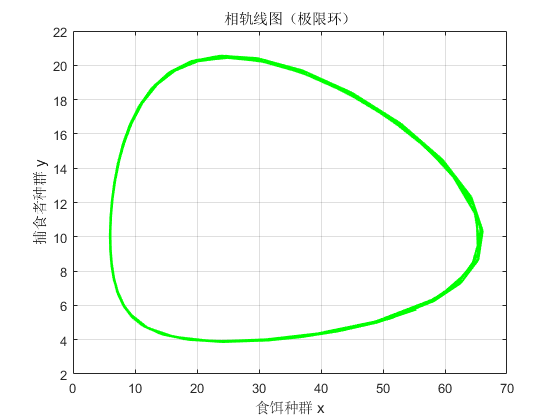
\includegraphics[width=0.49\textwidth]{figs/p2-004-001.png}
\caption{食饵—捕食者种群随时间变化（左）与相轨线图（极限环，右）}
\end{figure}

% ------------------------------------------------------------
\section{数模3插值与拟合}
% ------------------------------------------------------------

\subsection{题目 1：Lagrange 插值}
已知 $6$ 个观测点 $(x_i,y_i)$：$(1,16),(2,18),(3,21),(4,17),(5,15),(6,12)$，求插值函数
并估计 $x=1.5,2.6$ 处的值。Lagrange 插值基与插值多项式为
\[
l_k(x)=\prod_{\substack{j=0\\ j\neq k}}^{n}\frac{x-x_j}{x_k-x_j},\qquad
L_n(x)=\sum_{i=0}^{n}y_i\,l_i(x).
\]
求得
\[
\hat y=-\frac{29x^5}{120}+\frac{13x^4}{3}-\frac{695x^3}{24}+\frac{263x^2}{3}-\frac{579x}{5}+69,
\]
$\hat y(1.5)=\dfrac{3819}{256}$，$\hat y(2.6)=\dfrac{326322}{15625}$。

\begin{lstlisting}[language=Matlab]
clear; clc;
x_data = [1, 2, 3, 4, 5, 6]; y_data = [16,18,21,17,15,12];
y = LagrangeInterpolation(x_data, y_data)
subs(y,1.5)
subs(y,2.6)
function P = LagrangeInterpolation(x_data, y_data)
    syms x; n = length(x_data); P = sym(0);
    for i = 1:n
        L_i = sym(1);
        for j = 1:n
            if j ~= i
                L_i = L_i * (x - x_data(j)) / (x_data(i) - x_data(j));
            end
        end
        P = P + y_data(i) * L_i;     % 累加基函数与对应 y 值的乘积
    end
    P = simplify(P);
end
\end{lstlisting}

\begin{figure}[H]
\centering
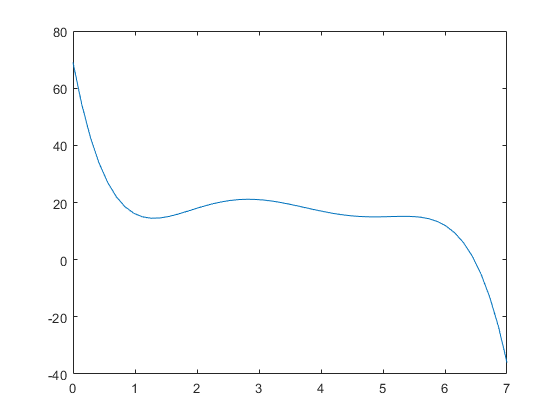
\includegraphics[width=0.55\textwidth]{figs/p3-002-000.png}
\caption{Lagrange 插值多项式曲线}
\end{figure}

\subsection{题目 2：三次样条}
速度曲线 $v(t)$ 的四个数据点为 $t=[0.15,0.16,0.17,0.18]$，$v=[3.5,1.5,2.5,2.8]$，
用三次样条插值求位移 $S=\int_{0.15}^{0.18}v(t)\dd t$。结果 $S=0.068625$。

\begin{lstlisting}[language=Matlab]
t = [0.15,0.16,0.17,0.18]; v = [3.5,1.5,2.5,2.8];
yy = spline(t, v);
S = integral(@(t) ppval(yy, t), 0.15, 0.18);
fprintf('位移 S = %.6f\n', S);
for i = 1:length(yy.breaks)-1
    a = yy.coefs(i,1); b = yy.coefs(i,2);
    c = yy.coefs(i,3); d = yy.coefs(i,4);
    fprintf('[%.2f, %.2f]: v(t) = %.4f t^3 + %.4f t^2 + %.4f t + %.4f\n',...
            yy.breaks(i), yy.breaks(i+1), a, b, c, d);
end
\end{lstlisting}

\subsection{题目 3：地图面积与边界}
以由西向东为 $x$ 轴、由南向北为 $y$ 轴，对某国地图等分测量南、北边界
$y_1,y_2$（单位 mm），数据如下。

\begin{table}[H]
\centering\footnotesize
\caption{某国国土地图边界测量值（单位：mm）}
\begin{tabular}{c*{14}{c}}
\toprule
$x$  & 7.0 & 10.5 & 13.0 & 17.5 & 34.0 & 40.5 & 44.5 & 48.0 & 56.0 & 61.0 & 68.5 & 76.5 & 80.5 & 91.0\\
$y_1$& 44 & 45 & 47 & 50 & 50 & 38 & 30 & 30 & 34 & 36 & 34 & 41 & 45 & 46\\
$y_2$& 44 & 59 & 70 & 72 & 93 & 100& 110& 110& 110& 117& 118& 116& 118& 118\\
\midrule
$x$  & 96.0 & 101.0 & 104.0 & 106.5 & 111.5 & 118.0 & 123.5 & 136.5 & 142.0 & 146.0 & 150.0 & 157.0 & 158.0 &\\
$y_1$& 43 & 37 & 33 & 28 & 32 & 65 & 55 & 54 & 52 & 50 & 66 & 66 & 68 &\\
$y_2$& 121& 124& 121& 121& 121& 122& 116& 83 & 81 & 82 & 86 & 85 & 68 &\\
\bottomrule
\end{tabular}
\end{table}

\textbf{问题分析：} 将南北边界视作 $x$ 的函数用三次样条拟合，对 $y_2-y_1$ 积分即得面积
（先作差再样条误差更小）。

\begin{lstlisting}[language=Matlab]
x  = [7.0,10.5,13.0,17.5,34.0,40.5,44.5,48.0,56.0,61.0,68.5,76.5,80.5,...
      91.0,96.0,101.0,104.0,106.5,111.5,118.0,123.5,136.5,142.0,146.0,...
      150.0,157.0,158.0];
y1 = [44,45,47,50,50,38,30,30,34,36,34,41,45,46,43,37,33,28,32,65,55,54,...
      52,50,66,66,68];
y2 = [44,59,70,72,93,100,110,110,110,117,118,116,118,118,121,124,121,121,...
      121,122,116,83,81,82,86,85,68];
x = x/18*40; y1 = y1/18*40; y2 = y2/18*40; y = y2 - y1;
ub = spline(x,y2); lb = spline(x,y1); yy = spline(x, y);
S = integral(@(x) ppval(yy, x), 5.0/18*40, 160.0/18*40)
xp = linspace(7.0/18*40, 158.0/18*40, 200);
plot(xp, ppval(yy,xp), '-'); hold on; plot(x, y, 'ro');
xlabel('x'); grid on;
\end{lstlisting}

\begin{figure}[H]
\centering
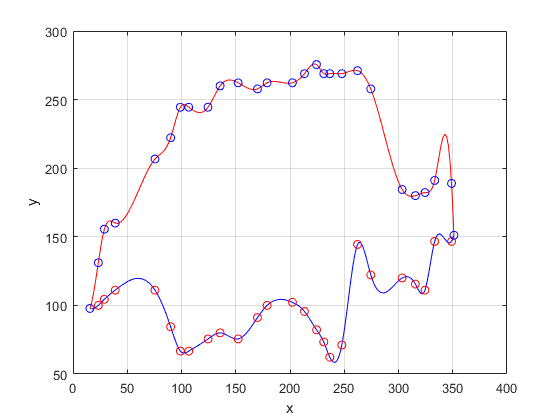
\includegraphics[width=0.6\textwidth]{figs/p3-005-001.png}
\caption{地图南、北边界的三次样条拟合}
\end{figure}

\subsection{题目 4：拟合模型比较}
根据数据拟合 $W=cg^3$ 与 $W=kgl^2$，比较优劣。

\begin{table}[H]
\centering\small
\begin{tabular}{c*{8}{c}}
\toprule
长度 $l$ & 14.5 & 12.5 & 17.25 & 14.5 & 12.625 & 17.75 & 14.125 & 12.625\\
腰围 $g$ & 9.75 & 8.375 & 11.0 & 9.75 & 8.5 & 12.5 & 9.0 & 8.5\\
体重 $W$ & 27 & 17 & 41 & 26 & 17 & 49 & 23 & 16\\
\bottomrule
\end{tabular}
\end{table}

用 \texttt{fitlm} 拟合，得模型 1：$c=0.0276,\ R^2=0.9467,\ \text{MSE}=7.7509$；
模型 2：$k=0.0126,\ R^2=0.9967,\ \text{MSE}=0.4841$。模型 2 的决定系数与方差均更优，为更佳模型。

\begin{lstlisting}[language=Matlab]
l = [14.5,12.5,17.25,14.5,12.625,17.75,14.125,12.625];
g = [9.75,8.375,11.0,9.75,8.5,12.5,9.0,8.5];
W = [27,17,41,26,17,49,23,16];
mdl1 = fitlm(g.^3, W, 'Intercept', false);      % W = c*g^3
mdl2 = fitlm(g.*(l.^2), W, 'Intercept', false); % W = k*g*l^2
fprintf('模型1: c=%.4f, R2=%.4f, MSE=%.4f\n',...
        mdl1.Coefficients.Estimate, mdl1.Rsquared.Ordinary, mdl1.MSE);
fprintf('模型2: k=%.4f, R2=%.4f, MSE=%.4f\n',...
        mdl2.Coefficients.Estimate, mdl2.Rsquared.Ordinary, mdl2.MSE);
\end{lstlisting}

\subsection{题目 5：二次型最小二乘}
对数据 $x=[0.1,0.2,0.3,0.4,0.5]$，$y=[0.06,0.12,0.36,0.65,0.95]$，
拟合 $y=c_1x^2+c_2x+c_3$，得 $c_1=3.7857,\ c_2=0.0386,\ c_3\approx0,\ R^2=0.9946$。

\begin{lstlisting}[language=Matlab]
x = [0.1,0.2,0.3,0.4,0.5]'; y = [0.06,0.12,0.36,0.65,0.95]';
X = [x.^2, x, ones(size(x))];
mdl = fitlm(X, y, 'Intercept', false);
c = mdl.Coefficients.Estimate;
fprintf('c1=%.4f, c2=%.4f, c3=%.4f, R2=%.4f\n', c(1),c(2),c(3), mdl.Rsquared.Ordinary);
\end{lstlisting}

\subsection{题目 6：非线性最小二乘}
对 $y=e^{-k_1x_1}\sin(k_2x_2)+x_3^2$ 拟合参数 $k_1,k_2\in[0,2]$（数据 25 组见下表）。
用 \texttt{lsqcurvefit} 得 $k_1\approx0,\ k_2\approx0.3099$，残差范数约 $56.21$。由于
$e^{-k_1x_1}\sin(k_2x_2)\in[-1,1]$ 而 $y-x_3^2$ 量级远大于此，拟合在区间端点附近达到最优
（$k_1$ 取下界 $0$ 使指数项保持为 $1$）。

\begin{table}[H]
\centering\footnotesize
\caption{非线性拟合数据（序号 / $y$ / $x_1$ / $x_2$ / $x_3$）}
\begin{tabular}{ccccc|ccccc}
\toprule
序号 & $y$ & $x_1$ & $x_2$ & $x_3$ & 序号 & $y$ & $x_1$ & $x_2$ & $x_3$\\
\midrule
1 &15.02&23.73&5.49&1.21 & 14&15.94&23.52&5.18&1.98\\
2 &12.62&22.34&4.32&1.35 & 15&14.33&21.86&4.86&1.59\\
3 &14.86&28.84&5.04&1.92 & 16&15.11&28.95&5.18&1.37\\
4 &13.98&27.67&4.72&1.49 & 17&13.81&24.53&4.88&1.39\\
5 &15.91&20.83&5.35&1.56 & 18&15.58&27.65&5.02&1.66\\
6 &12.47&22.27&4.27&1.50 & 19&15.85&27.29&5.55&1.70\\
7 &15.80&27.57&5.25&1.85 & 20&15.28&29.07&5.26&1.82\\
8 &14.32&28.01&4.62&1.51 & 21&16.40&32.47&5.18&1.75\\
9 &13.76&24.79&4.42&1.46 & 22&15.02&29.65&5.08&1.70\\
10&15.18&28.96&5.30&1.66 & 23&15.73&22.11&4.90&1.81\\
11&14.20&25.77&4.87&1.64 & 24&14.75&22.43&4.65&1.82\\
12&17.07&23.17&5.80&1.90 & 25&14.35&20.04&5.08&1.53\\
13&15.40&28.57&5.22&1.66 & & & & &\\
\bottomrule
\end{tabular}
\end{table}

\begin{lstlisting}[language=Matlab]
yfun = @(c,x) exp(-c(1)*x(:,1)) .* sin(c(2)*x(:,2)) + x(:,3).^2;
lb = zeros(1,2); ub = 2*ones(1,2);     % 主观设定参数上下界
c = lsqcurvefit(yfun, rand(1,2), x0, y0, lb, ub)
% c = [0.0000, 0.3099]，残差范数约 56.21
\end{lstlisting}

\subsection{题目 7：二元曲面拟合}
拟合 $z=\exp\!\Big(-\dfrac{(x-\mu_1)^2+(y-\mu_2)^2}{2\sigma^2}\Big)$。真值
$\mu_1=1,\mu_2=4,\sigma=6$，在网格上叠加标准正态噪声生成数据，分别用 \texttt{lsqcurvefit}
与 \texttt{fit} 拟合。两法结果基本一致：$c=(1.2416,3.1061,5.7014)$，均落在 $95\%$ 置信区间内。

\begin{lstlisting}[language=Matlab]
clc; clear; close all; rng(1)        % 固定随机数种子以保证可复现
x0 = linspace(-6,6,50); y0 = linspace(-5,5,60);
[X0,Y0] = meshgrid(x0,y0); XX0 = X0(:); YY0 = Y0(:);
zxy = @(c,xy) exp(-((xy(:,1)-c(1)).^2 + (xy(:,2)-c(2)).^2)/2/c(3)^2);
Z0 = zxy([1,4,6],[XX0,YY0]) + normrnd(0,1,size(XX0));   % 真值 + 噪声
c1 = lsqcurvefit(zxy, rand(1,3), [XX0,YY0], Z0)         % 方法一
ft = fittype('exp(-((x-mu1)^2+(y-mu2)^2)/2/s^2)',...
     'independent',{'x','y'},'dependent','z');
[c2, gof] = fit([XX0,YY0], Z0, ft, 'StartPoint', rand(3,1))  % 方法二
\end{lstlisting}

\begin{figure}[H]
\centering
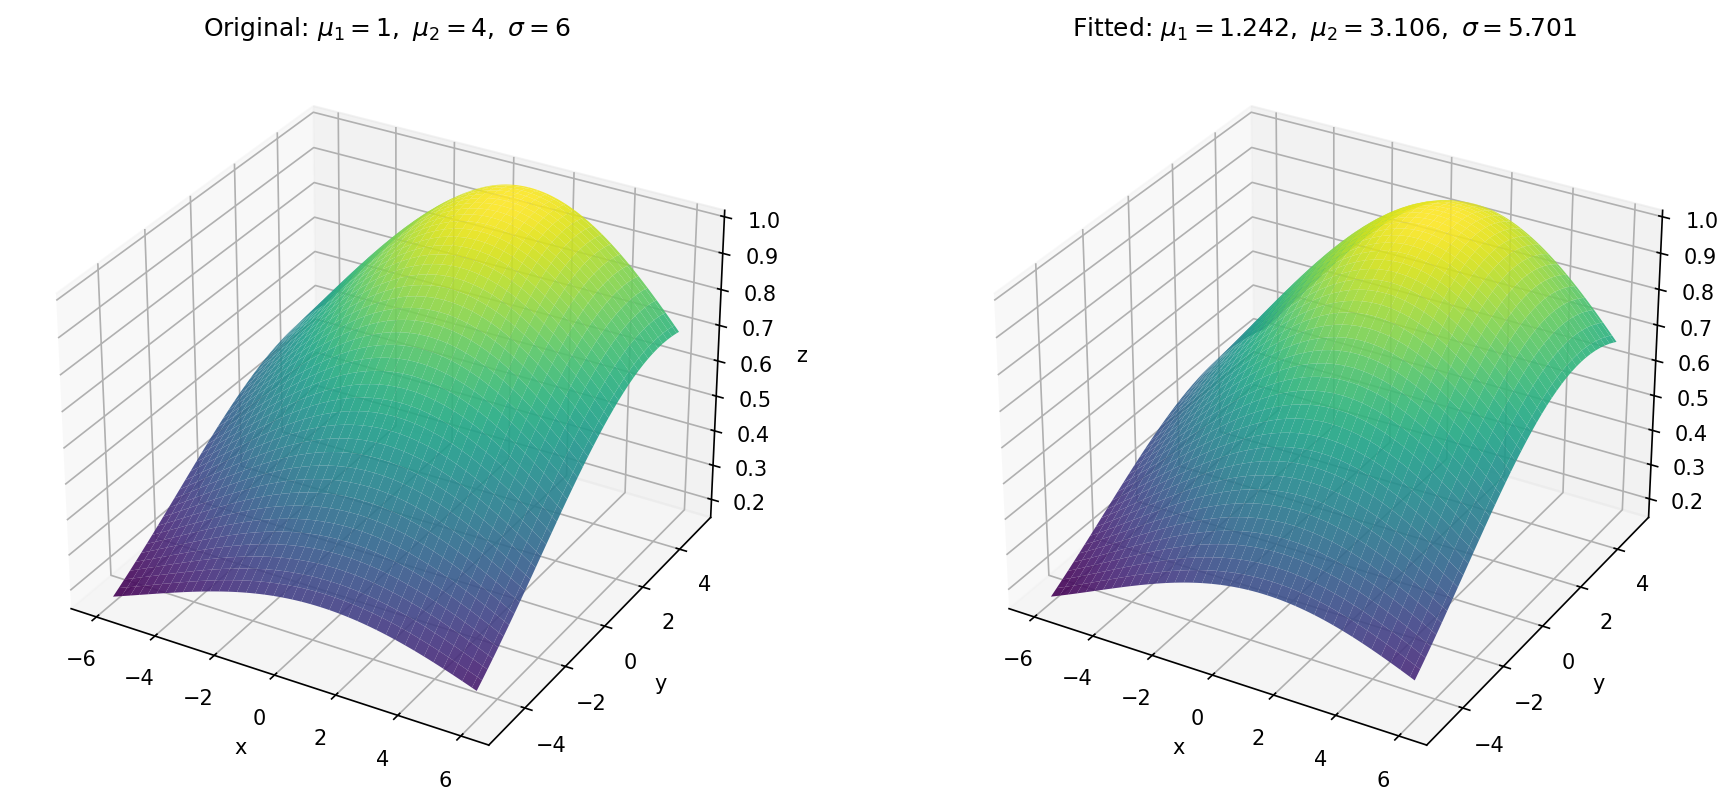
\includegraphics[width=0.8\textwidth]{figs/p3-010-002.png}
\caption{二元高斯曲面：原函数（左）与拟合曲面（右）对比}
\end{figure}

% ------------------------------------------------------------
\section{数模4蒙特卡洛}
% ------------------------------------------------------------

\subsection{题目 1：蒙特卡洛求面积}
用蒙特卡洛模拟近似求 $f(x)=\sqrt{x}\ (\tfrac12\le x\le\tfrac32)$ 下的面积。
该面积被矩形 $[\tfrac12,\tfrac32]\times[0,2]$ 包含。

\textbf{算法：}（1）计数器 $tot=0,\ cnt=0$；（2）在矩形内均匀产生 $(x,y)$，$tot{+}{+}$；
（3）若 $y^2\le x$ 则 $cnt{+}{+}$；（4）重复多次；（5）输出 $2\,cnt/tot$ 即面积近似值。
样本越多结果越准（$10^7$ 次约 $0.9889$）。

\begin{lstlisting}[language=C++]
#include<bits/stdc++.h>
using namespace std;
int cnt,tot,cs[11]={0,10,100,500,1000,5000,10000,50000,100000,5000000,10000000};
int main(){
    srand(time(0));
    for(int o=1;o<=10;o++){
        cnt=tot=0;
        for(int i=1;i<=cs[o];i++){
            double x=1.0*rand()/RAND_MAX+0.5;   // x in [0.5,1.5]
            double y=2.0*rand()/RAND_MAX;        // y in [0,2]
            tot++;
            if(y<pow(x,0.5)) cnt++;
        }
        printf("Testnumber=%d,S=%lf\n",cs[o],2.0*cnt/tot);
    }
    return 0;
}
\end{lstlisting}

\subsection{题目 2：二重积分}
求 $I=\iint_{x^2+y^2\le1}\sqrt{1-x^2}\dd x\dd y$。其几何意义为以圆为底、以 $\sqrt{1-x^2}$
为顶的几何体体积，被长方体 $[-1,1]\times[-1,1]\times[0,1]$ 包含，蒙特卡洛估计值约 $2.6667$
（真值 $8/3$）。

\begin{lstlisting}[language=C++]
#include<bits/stdc++.h>
using namespace std;
int cnt,tot,cs[11]={0,10,100,500,1000,5000,10000,50000,100000,5000000,500000000};
int main(){
    srand(time(0));
    for(int o=1;o<=10;o++){
        cnt=tot=0;
        for(int i=1;i<=cs[o];i++){
            double x=1.0*rand()/RAND_MAX*(rand()&1?1:-1);
            double y=1.0*rand()/RAND_MAX*(rand()&1?1:-1);
            double z=1.0*rand()/RAND_MAX;
            tot++;
            if(z*z<=1-x*x && x*x+y*y<=1) cnt++;
        }
        printf("Testnumber=%d,S=%lf\n",cs[o],4.0*cnt/tot);
    }
    return 0;
}
\end{lstlisting}

\subsection{题目 3：修理工排队系统}
单修理工，顾客到达间隔服从均值 $10$ min 的负指数分布，服务时间服从 $U[4,15]$ min，
先到先服务、队长无限、工作日 $8$ h。模拟结果：单个工作日完成 $36$ 人、平均等待
$6.57$ min；$1000$ 个工作日平均每日完成 $42.84$ 人、平均等待 $23.87$ min。

\begin{lstlisting}[language=Matlab]
[num1, avgWait1] = simulateOneDay();
fprintf('单日: 完成 %d 人, 平均等待 %.2f 分钟\n', num1, avgWait1);
N = 1000; totalCompleted = 0; totalAvgWait = 0;
for i = 1:N
    [num, avg] = simulateOneDay();
    totalCompleted = totalCompleted + num;
    totalAvgWait = totalAvgWait + avg;
end
fprintf('1000 日均: 完成 %.2f 人, 等待 %.2f 分钟\n', totalCompleted/N, totalAvgWait/N);

function [numCompleted, avgWait] = simulateOneDay()
    arrivalTimes = []; currentTime = 0;
    while true
        currentTime = currentTime + exprnd(10);  % 到达间隔 ~ 指数分布
        if currentTime > 480, break; end          % 超过 8 小时停止
        arrivalTimes(end+1) = currentTime;
    end
    numCompleted = 0; totalWait = 0; prevEnd = 0;
    for i = 1:length(arrivalTimes)
        arrival = arrivalTimes(i);
        service = unifrnd(4, 15);                  % 服务时间 ~ 均匀分布
        startTime = max(arrival, prevEnd);
        endTime = startTime + service;
        if endTime > 480, break; end
        numCompleted = numCompleted + 1;
        totalWait = totalWait + (startTime - arrival);
        prevEnd = endTime;
    end
    if numCompleted == 0, avgWait = 0;
    else, avgWait = totalWait / numCompleted; end
end
\end{lstlisting}

% ------------------------------------------------------------
\section{数模5多目标规划}
% ------------------------------------------------------------

\subsection{题目 1：生产计划（线性规划）}
某厂用 5 道工序（I--V）生产 3 种产品，设备费用按"实际占用台时与有效台时之比"线性分摊。
设日产量 $x_1,x_2,x_3$，模型为
\[
\max z=\sum_{i=1}^{3}(p_i-r_i)x_i-\sum_{k=1}^{5}\frac{c_k}{T_k}\sum_{i=1}^{3}a_{ki}x_i,
\quad
\text{s.t.}\ \sum_{i=1}^{3}a_{ki}x_i\le T_k,\ x_i\ge0.
\]
计算得净利润系数 $\approx(-0.297,-1.220,1.915)$，产品 1、2 边际利润为负故 $x_1=x_2=0$；
产品 3 仅受工序 II 约束 $12x_3\le10000$，得 $x_3\approx833.33$，最大利润 $\approx1595.67$ 元/日。

\begin{lstlisting}[language=Matlab]
clc; clear;
p = [1.25 2.00 2.80]; r = [0.25 0.35 0.50];     % 售价、原料成本
a = [5 10 0; 7 9 12; 6 8 0; 4 11 0; 0 7 0];     % 各工序单位台时
T = [6000;10000;4000;7000;4000];                % 有效台时
c = [300;321;250;783;200];                      % 满负荷费用
f = -((p - r)' - a' * (c ./ T));                % linprog 求 min，故取负
[x, fval] = linprog(f, a, T, [], [], [0;0;0]);
fprintf('产量 x = [%.2f %.2f %.2f]\n', x);
fprintf('最大利润 = %.2f 元/日\n', -fval);
% 非线性扩展：若设备一经启用即付全部满负荷费，引入 0-1 变量 y_k，
% 目标改为 sum((p-r)x) - sum(c_k y_k)，并加大 M 约束 sum a_ki x_i <= T_k y_k，
% 成为混合整数规划，用 intlinprog 求解。
\end{lstlisting}

\subsection{题目 2：选址问题（非线性规划）}
6 个工地坐标 $(a_i,b_i)$ 与日用量 $d_i$ 已知，临时料场 $A(5,1),B(2,7)$，各储量 20 t。

\textbf{（1）料场位置已知——线性规划：} 设 $x_{ij}$ 为料场 $j$ 运往工地 $i$ 的水泥量，
$D_{ij}$ 为欧氏距离，
\[
\min\sum_{i=1}^{6}\sum_{j=1}^{2}D_{ij}x_{ij},\quad
\text{s.t.}\ \sum_{j}x_{ij}=d_i,\ \sum_{i}x_{ij}\le20,\ x_{ij}\ge0.
\]
最优总吨公里数为 $137.07$。

\textbf{（2）同时优化料场位置——非线性规划：} 未知量为 $\{x_{ij}\}$ 与料场坐标
$(\alpha_j,\beta_j)$ 共 16 个，$D_{ij}=\sqrt{(a_i-\alpha_j)^2+(b_i-\beta_j)^2}$ 为非线性，
用 \texttt{fmincon} 并以第（1）问解作初值。结果总吨公里数由 $137.07$ 降至 $89.88$（下降约 $34\%$）。
注：非凸问题应取多组随机初值取最优。

\begin{lstlisting}[language=Matlab]
a = [1.25 8.75 0.50 3.75 3.00 7.25];
b = [1.25 0.75 4.75 5.00 6.50 7.75];
d = [3 5 4 7 6 11];
% ---- (1) 料场位置固定的线性规划 ----
loc = [5 1; 2 7]; D = zeros(6,2);
for i = 1:6, for j = 1:2, D(i,j) = norm([a(i) b(i)] - loc(j,:)); end; end
f = D(:);
Aeq = zeros(6,12); for i = 1:6, Aeq(i,i) = 1; Aeq(i,i+6) = 1; end
beq = d';
Acap = zeros(2,12); Acap(1,1:6) = 1; Acap(2,7:12) = 1;
[x1, fv1] = linprog(f, Acap, [20;20], Aeq, beq, zeros(12,1));
fprintf('(1) 最小吨公里数 = %.2f\n', fv1);
% ---- (2) 同时优化料场坐标的非线性规划 ----
obj = @(v) totalTonKm(v, a, b);     % v = [x(1:12); ax1 ay1 ax2 ay2]
v0 = [x1; 5;1;2;7];
Aeq2 = [Aeq, zeros(6,4)];
v = fmincon(obj, v0, [], [], Aeq2, beq, [zeros(12,1);-inf(4,1)], []);
fprintf('(2) 最小吨公里数 = %.2f\n', obj(v));

function s = totalTonKm(v, a, b)
    x = reshape(v(1:12),6,2);
    P = [v(13) v(14); v(15) v(16)]; s = 0;
    for i = 1:6, for j = 1:2
        s = s + x(i,j) * norm([a(i) b(i)] - P(j,:));
    end; end
end
\end{lstlisting}

\subsection{题目 3：飞行管理问题（非线性规划）}
$160$ km 见方空域内若干飞机水平匀速飞行（$v=800$ km/h），要求任意两机始终保持
$\ge8$ km 安全距离，调整方向角且幅度尽量小（$\le0.01^\circ$）。设调整量 $\Delta\theta_i$，
调整后 $\alpha_i=\theta_i+\Delta\theta_i$，两机相对位移 $\Delta r_{ij}(t)=\Delta p+t\Delta v$，
其中 $\Delta p=(x_i-x_j,y_i-y_j),\ \Delta v=v(\cos\alpha_i-\cos\alpha_j,\sin\alpha_i-\sin\alpha_j)$。
最小距离平方
\[
d_{ij,\min}^2=
\begin{cases}
|\Delta p|^2-\dfrac{(\Delta p\cdot\Delta v)^2}{|\Delta v|^2}, & \Delta p\cdot\Delta v<0,\\[2mm]
|\Delta p|^2, & \text{否则}.
\end{cases}
\]
优化模型 $\min\sum_i\Delta\theta_i^2$，s.t. $d_{ij,\min}^2\ge8^2,\ |\Delta\theta_i|\le\pi/6$。
原始轨迹下 $(3,6)$ 对最小距离约 $4.4$ km 为主要冲突；优化后只需飞机 3 转角增加约
$1.19^\circ$、新进入飞机 6 增加约 $1.59^\circ$，即可使所有两机距离 $\ge8$ km。

\begin{lstlisting}[language=Matlab]
clc; clear;
x = [150 85 150 145 130 0]; y = [140 85 155 50 150 0];
th = deg2rad([243 236 220.5 159 230 52]); v = 800; n = 6;
obj = @(dth) sum(dth.^2);
nonl = @(dth) flightCon(dth, x, y, th, v, n);
lb = -pi/6*ones(1,n); ub = pi/6*ones(1,n);
dtheta = fmincon(obj, zeros(1,n), [], [], [], [], lb, ub, nonl);
fprintf('方向角调整量 (度): '); disp(rad2deg(dtheta));

function [c,ceq] = flightCon(dth, x, y, th, v, n)
    a = th + dth; ceq = []; c = [];
    for i = 1:n-1, for j = i+1:n
        dp = [x(i)-x(j), y(i)-y(j)];
        dv = v*[cos(a(i))-cos(a(j)), sin(a(i))-sin(a(j))];
        if dot(dp,dv) < 0
            d2 = dp*dp' - (dp*dv')^2/(dv*dv');
        else
            d2 = dp*dp';
        end
        c(end+1) = 8^2 - d2;     % 要求 d2 >= 64
    end; end
end
\end{lstlisting}

\subsection{题目 4：多目标规划}
产品 A、B 月产量 $x_1,x_2$，需求 $x_1+x_2\ge9$，产能 $x_1\le5,x_2\le8$：
\[
\min f_1=2100x_1+4800x_2,\qquad \max f_2=3600x_1+6500x_2.
\]
可行域顶点 $(5,4),(5,8),(1,8)$。单目标极值给出 Pareto 前沿端点：极小投资点 $(5,4)$
投资 $29700$、利润 $44000$；极大利润点 $(5,8)$ 投资 $48900$、利润 $70000$。
线性加权法临界权重 $w^*\approx0.486$。$\varepsilon$-约束法可精确刻画前沿：给定利润目标
$\varepsilon\in[44000,70000]$，最优解恒有 $x_1=5,\ x_2=(\varepsilon-18000)/6500$，
即前沿为线段 $\{(5,x_2)\mid4\le x_2\le8\}$。多得 1 元利润对应增加 $4800/6500\approx0.738$ 元投资。

\begin{lstlisting}[language=Matlab]
A = [-1 -1]; bcon = -9;          % x1 + x2 >= 9
lb = [0 0]; ub = [5 8];
% 端点1：最小投资
[~, f1min] = linprog([2100 4800], A, bcon, [], [], lb, ub);
% 端点2：最大利润
[~, f2max] = linprog([-3600 -6500], A, bcon, [], [], lb, ub);
fprintf('最小投资 = %.0f, 最大利润 = %.0f\n', f1min, -f2max);
% epsilon-约束法刻画 Pareto 前沿
for eps = 44000:5000:70000
    [x,fv] = linprog([2100 4800], [A; -3600 -6500], [bcon; -eps], [], [], lb, ub);
    fprintf('eps=%5d: x=(%.2f,%.2f), 投资=%.0f\n', eps, x(1), x(2), fv);
end
\end{lstlisting}

% ------------------------------------------------------------
\section{数模6图论建模}
% ------------------------------------------------------------

\subsection{题目 1：设备更新问题}
某公司第一年初购入设备，5 年内使总费用最省。设备价格与维修费如下。

\begin{table}[H]
\centering\small
\begin{tabular}{lccccc}
\toprule
年 & 1 & 2 & 3 & 4 & 5\\
价格 & 11 & 11 & 12 & 12 & 13\\
\midrule
使用年限 & 0--1 & 1--2 & 2--3 & 3--4 & 4--5\\
维修费用 & 5 & 6 & 8 & 11 & 18\\
\bottomrule
\end{tabular}
\end{table}

\textbf{建模：} 构造有向图 $G=(V,E)$，$V=\{0,1,2,3,4,5\}$ 表示各年初；边 $(i,j)$ 表示第
$i$ 年购入用到第 $j$ 年初，权值
\[
c_{ij}=p_i+\sum_{k=i}^{j-1}r_k.
\]
定义 $f(j)$ 为第 0 年到第 $j$ 年最小费用，$f(j)=\min_{0\le i<j}\{f(i)+c_{ij}\},\ f(0)=0$。逐年递推：
\[
\begin{aligned}
f(1)&=16,\quad f(2)=22,\quad f(3)=30,\quad f(4)=41,\\
f(5)&=\min(59,57,53,53,59)=53.
\end{aligned}
\]
回溯得最优方案：第 0 年购入用至第 2 年（费用 22），第 2 年再购入用至第 5 年（费用 31），
总费用 $f(5)=53$。

\subsection{题目 2：minimax 选址问题}
连锁企业 6 个销售点构成交通网络（边权为公路距离），求使"离仓库最远销售点路程最短"的
建仓位置。

\begin{figure}[H]
\centering
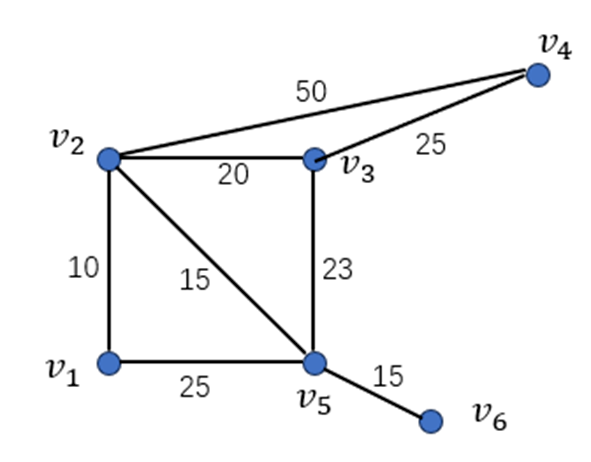
\includegraphics[width=0.5\textwidth]{figs/p6-003-000.png}
\caption{销售点交通网络图（边权为公路距离）}
\end{figure}

由邻接矩阵 $D$（无连接记 $\infty$），用 Floyd--Warshall 求全部点对最短路，统计每个顶点
作仓库时到其他点的最大最短路：
\[
v_1{:}55,\ v_2{:}45,\ v_3{:}38,\ v_4{:}63,\ v_5{:}48,\ v_6{:}63.
\]
最优选址为 $v_3$，最坏距离 $38$ 为所有点中最小。

\begin{lstlisting}[language=Python]
import networkx as nx
G = nx.Graph()
edges = [("v1","v2",10),("v1","v5",25),("v2","v3",20),("v2","v4",50),
         ("v2","v5",15),("v3","v4",25),("v3","v5",23),("v5","v6",15)]
G.add_weighted_edges_from(edges)
shortest = dict(nx.all_pairs_dijkstra_path_length(G))
max_dist = {n: max(d.values()) for n, d in shortest.items()}
center = min(max_dist, key=max_dist.get)
print(max_dist, center, max_dist[center])
\end{lstlisting}

\subsection{题目 3：最大流}
求源 $v_1$ 到汇 $v_6$ 的最大流。设边 $(i,j)$ 容量 $c_{ij}$、流量 $x_{ij}$，
\[
\max\ x_{12}+x_{13},\quad \text{s.t. } 0\le x_{ij}\le c_{ij},\ \text{各中间节点流量守恒}.
\]
求得最大流值 $=10$，一组最优流为 $x_{12}=8,x_{13}=2,x_{23}=3,x_{24}=5,x_{35}=5,x_{46}=5,x_{56}=5$。

\begin{figure}[H]
\centering
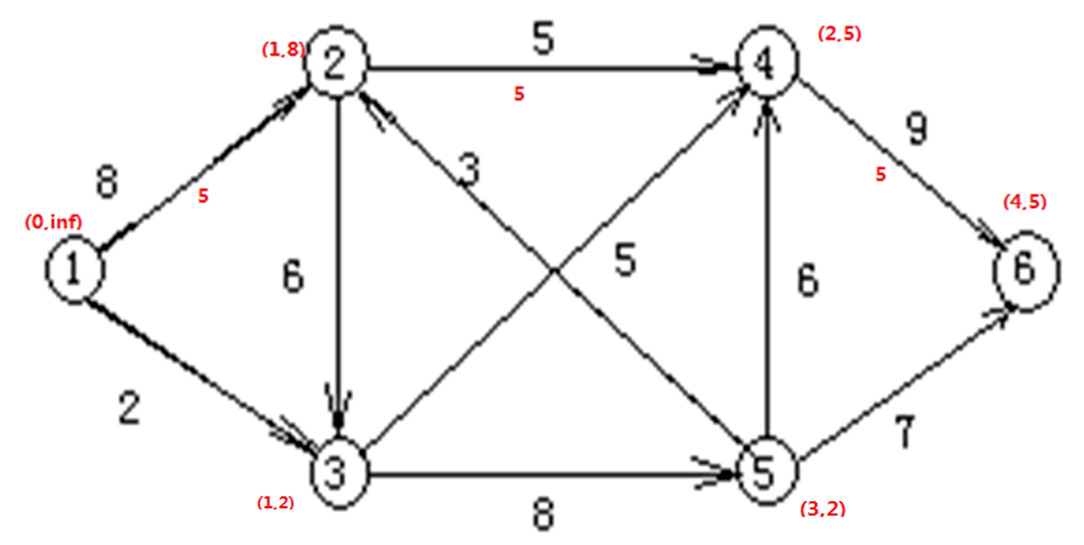
\includegraphics[width=0.6\textwidth]{figs/p6-005-002.png}
\caption{最大流网络图（黑色为容量，红色为最优流量）}
\end{figure}

% ------------------------------------------------------------
\section{数模7概率统计建模}
% ------------------------------------------------------------

\subsection{题目 1：吸收马氏链转移概率}
给定吸收链转移概率矩阵（图~\ref{fig:trans}），求平均转移次数与落入各吸收状态的概率。

\begin{figure}[H]
\centering
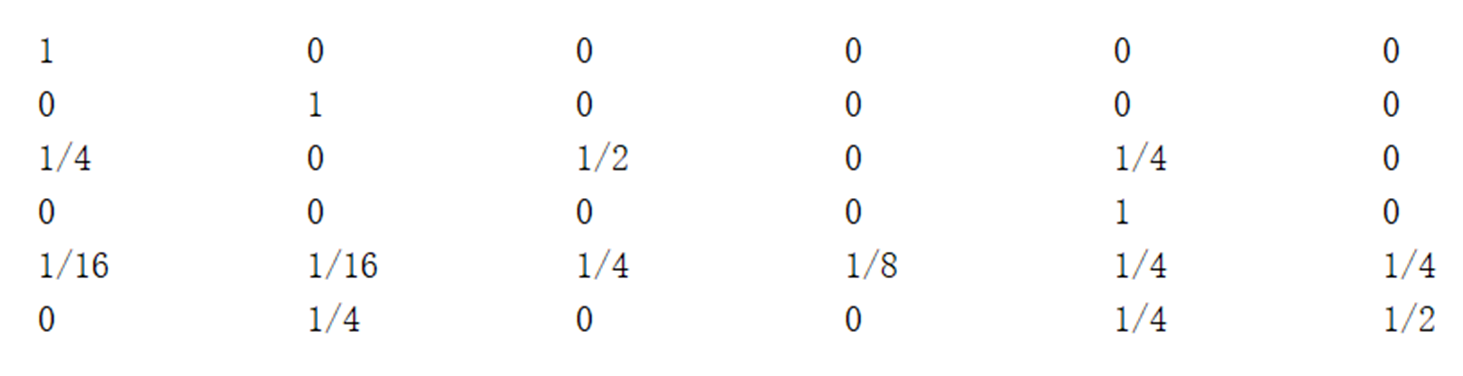
\includegraphics[width=0.85\textwidth]{figs/p7-001-000.png}
\caption{吸收马氏链转移概率矩阵}
\label{fig:trans}
\end{figure}

将矩阵分块 $P=\begin{pmatrix}I&0\\ R&Q\end{pmatrix}$，基本矩阵 $N=(I-Q)^{-1}$，
吸收概率 $B=NR$。从瞬时状态 $2,4,5$ 出发的平均转移次数均为 $4$ 步；落入吸收状态 $0,1,3$ 的概率
\[
B=\begin{pmatrix}
0.6875 & 0.1875 & 0.125\\
0.375 & 0.375 & 0.25\\
0.1875 & 0.6875 & 0.125
\end{pmatrix}.
\]

\begin{lstlisting}[language=Python]
import numpy as np
P = np.array([
    [1,0,0,0,0,0],
    [0,1,0,0,0,0],
    [1/4,0,1/2,0,1/4,0],
    [0,0,0,1,0,0],
    [1/16,1/16,1/4,1/8,1/4,1/4],
    [0,1/4,0,0,1/4,1/2]])
Q = P[:4,:4]; R = P[:4,4:]
N = np.eye(4) - Q
mu = np.linalg.inv(np.eye(4) - N)        # 平均转移次数
pi = np.linalg.inv(np.eye(4) - Q) @ R    # 落入各吸收状态的概率
print("mu:\n", mu); print("pi:\n", pi)
\end{lstlisting}

\subsection{题目 2：多元统计回归（猪胴体性状）}
对 25 头育肥猪，作瘦肉量 $y$ 对眼肌面积 $x_1$、腿肉量 $x_2$、腰肉量 $x_3$ 的多元回归。

\begin{figure}[H]
\centering
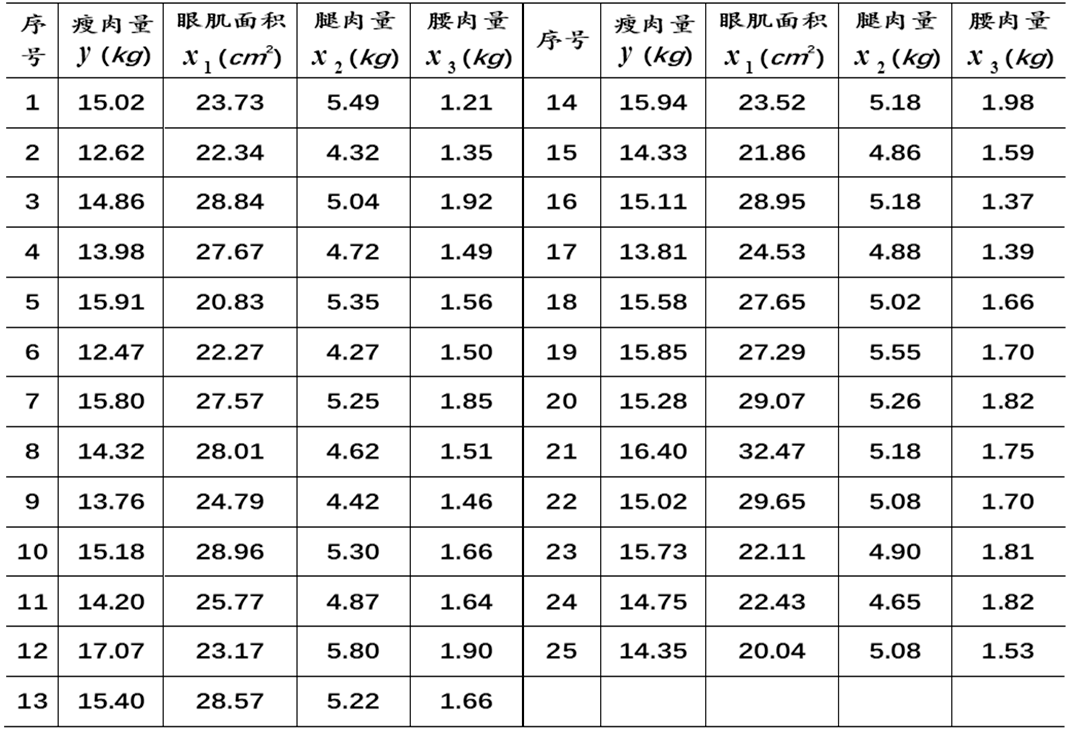
\includegraphics[width=0.85\textwidth]{figs/p7-003-002.png}
\caption{25 头育肥猪的 4 个胴体性状数据}
\end{figure}

OLS 拟合得 $R^2=0.844$（调整 $R^2=0.821$，$F=37.75$）。回归系数中 $x_2,x_3$ 显著
（$p<0.01$），$x_1$ 不显著（$p=0.549$）：
\[
\hat y=0.8539+0.0178x_1+2.0782x_2+1.9396x_3.
\]

\begin{lstlisting}[language=Python]
import numpy as np, pandas as pd, statsmodels.api as sm
import matplotlib.pyplot as plt
df = pd.DataFrame({'y':[...], 'x1':[...], 'x2':[...], 'x3':[...]})  # 见上表
X = sm.add_constant(df[['x1','x2','x3']]); y = df['y']
model = sm.OLS(y, X).fit()
print(model.summary())
# 残差图
plt.scatter(model.fittedvalues, model.resid)
plt.axhline(0, color='red', linestyle='--')
plt.xlabel('Fitted values'); plt.ylabel('Residuals'); plt.show()
# 二项式（含平方项）回归并比较
X_poly = np.column_stack((df.x1, df.x2, df.x3, df.x1**2, df.x2**2, df.x3**2))
model_poly = sm.OLS(y, sm.add_constant(X_poly)).fit()
print("Linear R2:", model.rsquared, " Poly R2:", model_poly.rsquared)
\end{lstlisting}

\subsection{题目 3：蠓虫分类判别}
已知 6 个 Apf 蠓虫与 9 个 Af 蠓虫的触角长、翅长，建立判别模型区分两类，并识别 3 个待判样本。

\begin{figure}[H]
\centering
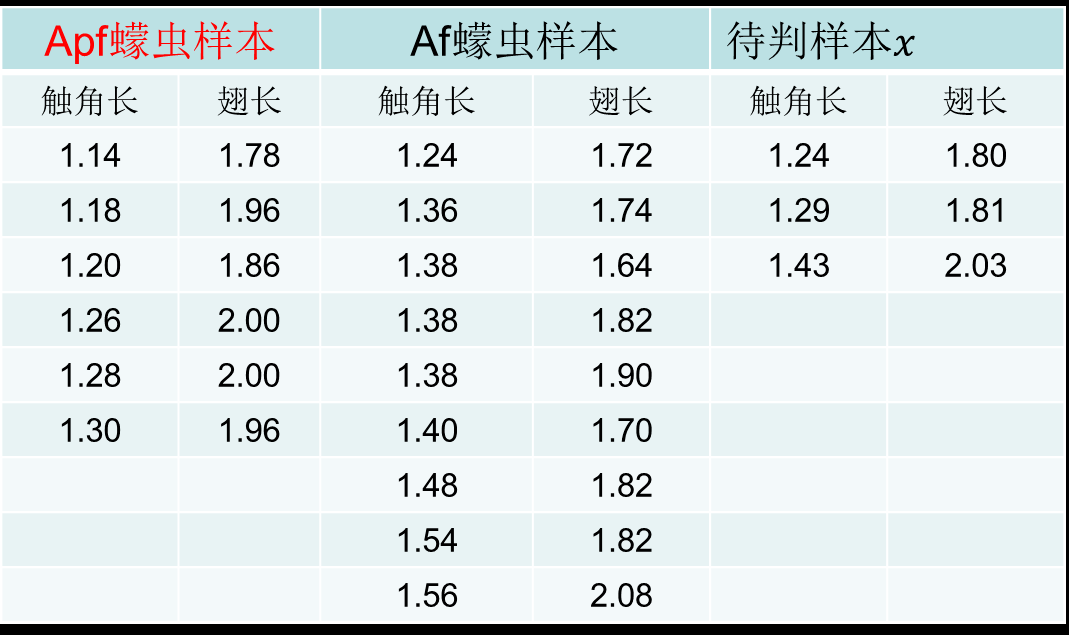
\includegraphics[width=0.7\textwidth]{figs/p7-006-004.png}
\caption{Apf / Af 蠓虫及待判样本的触角长与翅长}
\end{figure}

用线性判别分析（LDA），对待判样本 $(1.24,1.80),(1.29,1.81),(1.43,2.03)$ 的预测类别为
$[0,1,1]$（$0=$Apf，$1=$Af）。若 Apf 为毒蠓、Af 为益蠓，则应调整误判代价：宁可将益蠓
误判为毒蠓（降低漏检毒蠓的风险），即在判别时提高判为 Apf 的先验/代价权重。

\begin{lstlisting}[language=Python]
import numpy as np
from sklearn.discriminant_analysis import LinearDiscriminantAnalysis as LDA
X = np.array([[1.14,1.78],[1.18,1.96],[1.20,1.86],[1.26,2.00],[1.28,2.00],
              [1.30,1.96],[1.24,1.72],[1.36,1.74],[1.38,1.64],[1.38,1.82],
              [1.40,1.90],[1.48,1.82],[1.54,1.82],[1.56,2.08]])
y = np.array([0,0,0,0,0,0,1,1,1,1,1,1,1,1])    # Apf=0, Af=1
lda = LDA(); lda.fit(X, y)
samples = np.array([[1.24,1.80],[1.29,1.81],[1.43,2.03]])
print("预测类别：", lda.predict(samples))       # [0 1 1]
\end{lstlisting}

\end{document}
